% !TeX root = RJwrapper.tex
\title{R as Platform for the Analysis of dPCR and qPCR Experiments}
\author{by Stefan R\"{o}diger, Micha\l{} Burdukiewicz, Konstantin 
Blagodatskikh and Peter Schierack}

\maketitle

\abstract{
There is an ever-increasing number of applications, which use quantitative PCR 
(qPCR) or digital PCR (dPCR) to elicit fundamentals of biological processes. 
Novel amplification strategies based on quantitative isothermal amplification 
(qIA) become more prominent in life sciences and diagnostics. Several software 
solutions have been developed, which are either distributed as closed source 
software or as monolithic block with little freedom to perform highly customized 
analysis procedures. Others and we argue that R is an excellent environment for 
a reproducible and transparent analysis of data. However, for newcomers it is 
often very challenging to master R from reading the manuals and FAQs the not 
obvious steps. Here we describe exemplary workflows for the analysis of dPCR, 
qIA or qPCR experiments including the analysis of melting curve data. Our 
analysis relies entirely on R packages available from public repositories.
}

\section{Introduction}

The qPCR is the method of choice when a precise quantification of minute DNA 
traces of pathogens or the analysis of gene expression is required 
\citep{peirson_2003}. Numerous commercial and experimental monitoring platforms 
have been developed in the past years. This includes standard plate cyclers, 
capillary cyclers, microfluidic platforms and related technologies 
\citep{rodiger_highly_2013, devonshire_2013, viturro_2014, rodiger_nucleic_2014, 
khodakov_2014}. Only few bioanalytical applications had such a significant 
impact on the progress of life sciences and medical sciences as the quantitative 
Polymerase Chain Reaction (qPCR). The scientific community work hard in the past 
two decades to uncover pitfalls of qPCR experiments. This lead finally to the 
development of peer-reviewed analysis algorithms \citep{ruijter_2013}, 
throughout analysed qPCR chemistries \citep{ruijter_2014} and guidelines for a 
proper conduct of qPCR experiments as implemented in the MIQE guidelines 
(minimum information for publication of quantitative real-time PCR experiments) 
\citep{bustin_miqe_2009, huggett_2013}. In the past decades 
emerged several isothermal amplification technologies, such as helicase 
dependent amplification (HDA), as alternative to PCR. Isothermal amplification 
was readily combined with real-time monitoring technologies (qIA) and is used 
nowadays in various fields like diagnostics and point of care testing 
\citep{rodiger_nucleic_2014}.

Digital PCR (dpcR) is a novel approach for detection and quantification of 
nucleic acids. The dPCR Technology breaks fundamentally with the previous 
concept of nucleic acid quantification and can be seen as a next generation 
nucleic acid quantification. The key difference between dPCR and traditional PCR 
lies in the method of measuring (absolute) nucleic acids amounts, which yields 
discrete information instead of the continuous signal. This is possible after 
``clonal DNA amplification'' in thousands of small separated partitions (e.g., 
droplets, nano chambers) \citep{huggett_2013, milbury_2014, morley_2014}. 
Partitions with no nucleic acid remain negative and the others turn positive 
(e.g., Figure~\ref{figure:dpcR_sim}). Selected technologies (e.g., 
OpenArray\textregistered Real-Time PCR System) monitor amplification reactions 
in the chambers in real-time. Cq values are calculated from the amplification 
curves and converted into discrete events by means of positive and negative 
partitions and the absolute quantification of nucleic acids is done using 
Poisson distribution. Recently we published the \CRANpkg{dpcR} package at CRAN, which is the first 
open source software package based on R for the analysis of digital PCR (dPCR) 
experiments (see \CRANpkg{dpcR} for details).

\begin{figure}[htbp]
  \centering
  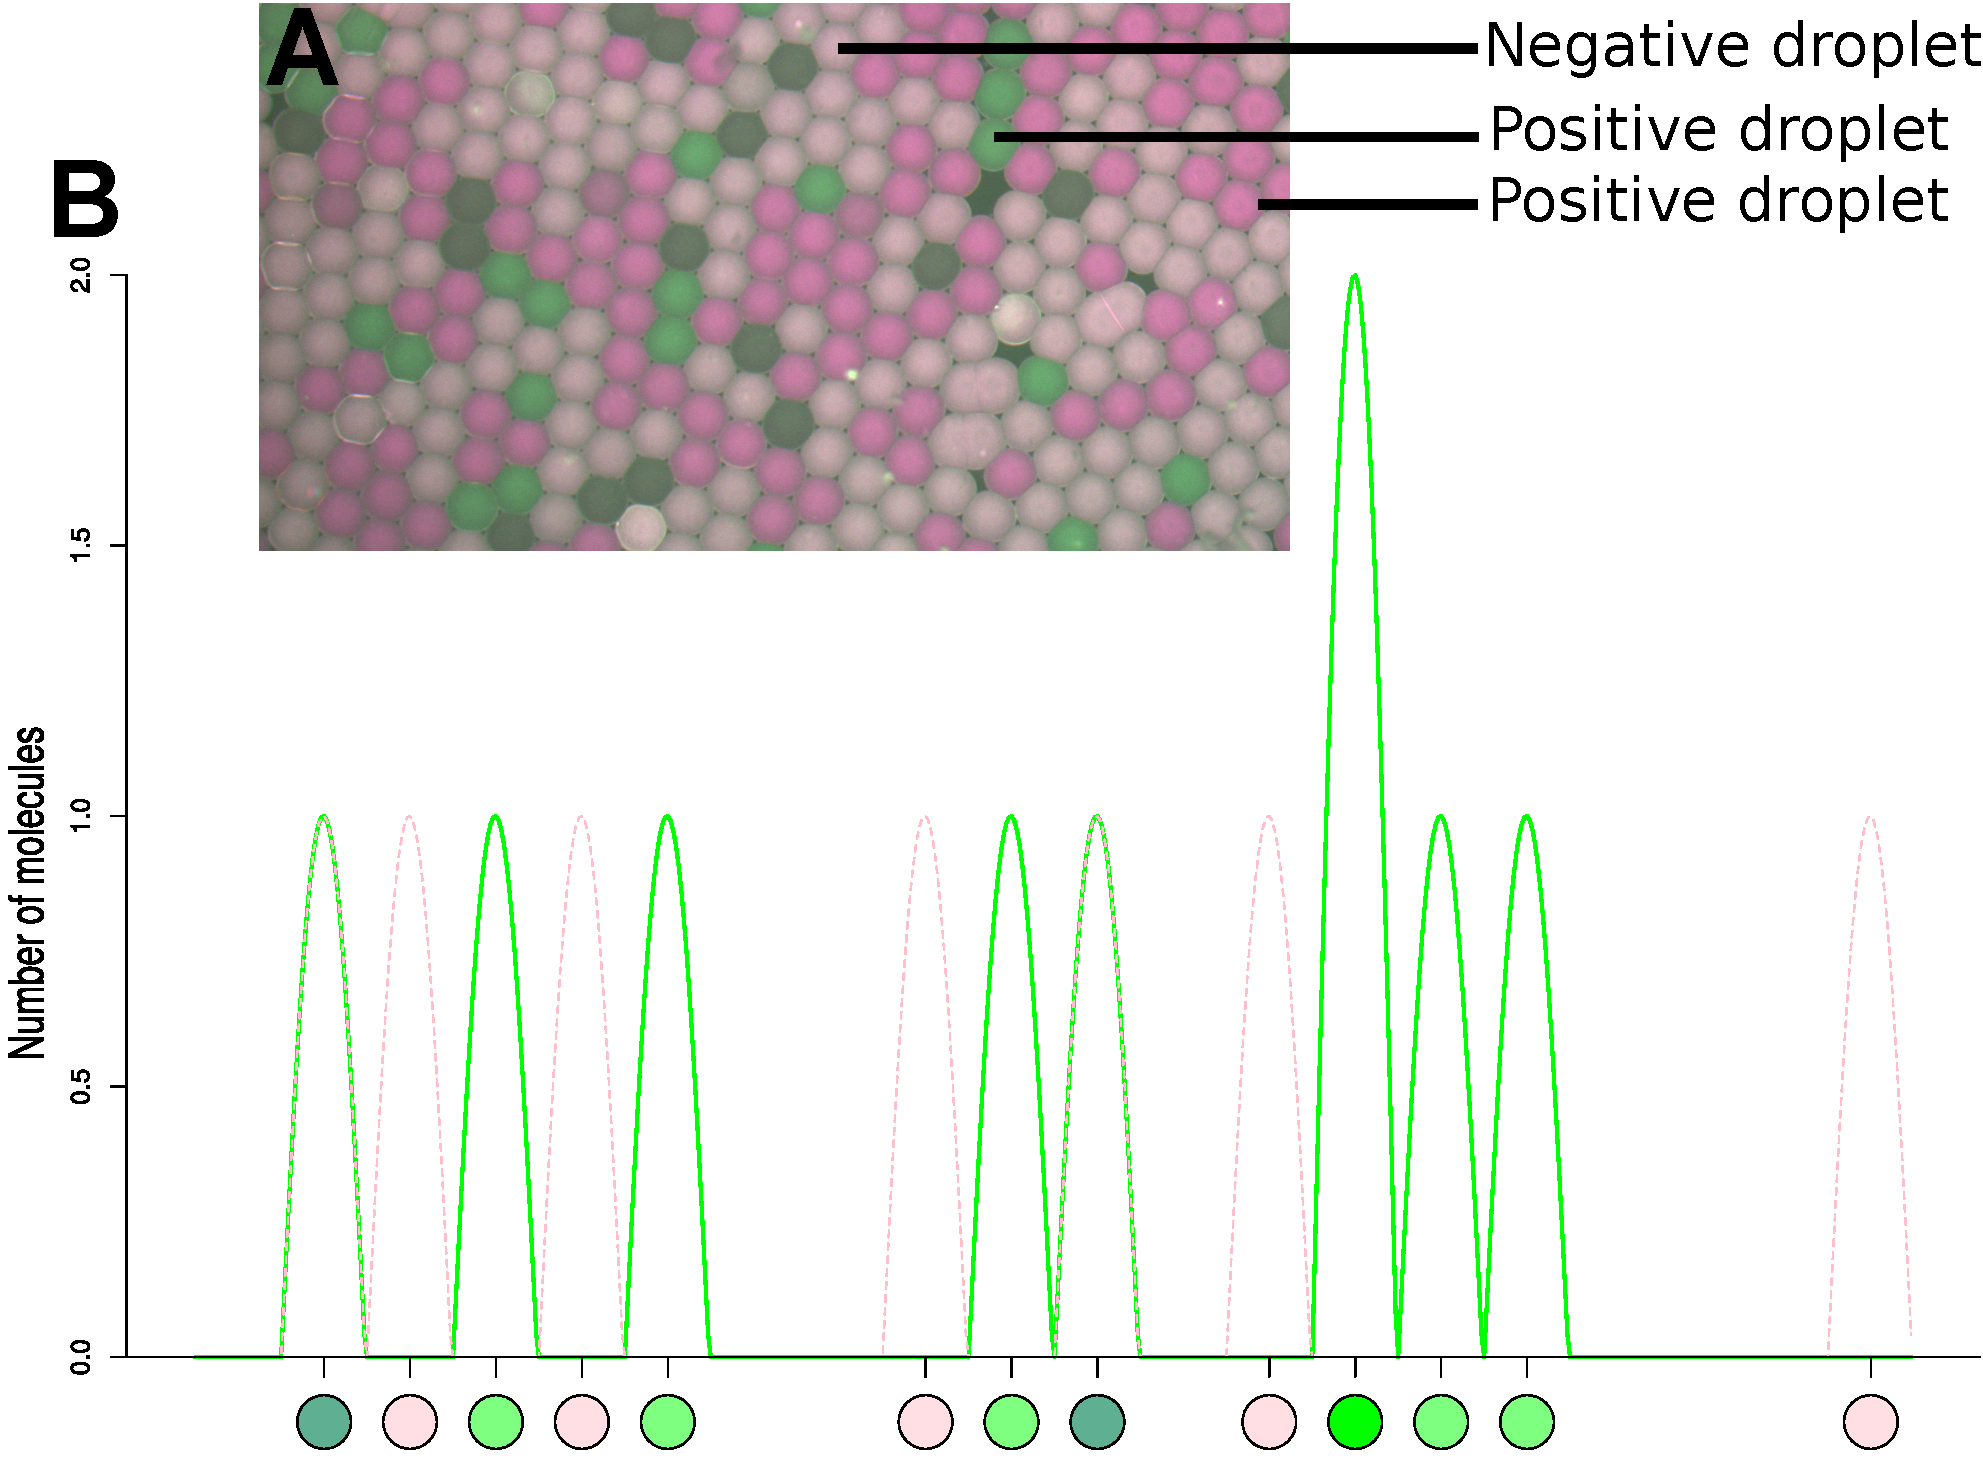
\includegraphics[clip=true, width=14cm]{figures/dpcR_sim.pdf}
  \caption{Scheme of droplet digital PCR experiment. \strong{A)} A droplet 
digital PCR reaction mix was formed in a Bio-Rad QX100 system. The droplets 
(circa 100 $\mu$m in diameter) were subjected to the VideoScan platform for 
detection and analysis. \strong{(B)} Subsequently the samples can be digitalized 
by counting number of positive and total number of droplets.}
\label{figure:dpcR_sim}
\end{figure}

Most of the commercial and experimental hardware platforms provide means to 
analyse the amplification curve data. Yet, in case of closed source software the 
analysis happens in most cases in a blackbox fashion tied to a specific 
platforms. Often such systems have limitation in the data processing and force 
the used to suboptimal analysis algorithm as discussed by \citet{ruijter_2013}. 
The visualization options are usually limited by the software and not in 
acceptable publication quality. The data processing in spreadsheets is not advisable 
for research purposes. Often lacking tools to validate input, debug implemented procedures
and automatize worflow spreadsheets are prone to errors and not well suited for more
complicated analysis\footnote{For more elaborated critique see 
\url{http://www.burns-stat.com/documents/tutorials/spreadsheet-addiction/} 
and \citet{mccullough_2008}.}.

The complexity of hardware, wetware and software requires expertise to master a 
technical workflow comprising standards for experimental design, generation and 
analysis of data, interpretation of results and reporting 
\citep{huggett_BDQ_2014}. We argue that blackboxs are not necessarily a bad 
thing, but should be avoided wherever possible. Studies by 
\citet{mccullough_2008, Almiron_2010, Duran_2014} exemplified this. Scientific 
misconduct and fraud have shaken the scientific community on several occasions 
\citep{fang_2012}. In particular qPCR is a sensible topic.

R is one of the most used tools in 
bioinformatics and is known as an early adopter of emerging technologies 
\citep{pabinger_2014} due to several reasons. R provides essential packages to 
build a highly customized workflows, covering: data read-in, data preprocessing, 
analysis, post-processing, visualization and storage. As recently briefly 
reviewed in \citet{pabinger_2014}, numerous R packages have been developed for 
the analysis of qPCR experiments, including: \CRANpkg{kulife}, 
\CRANpkg{MCMC.qpcr}, \CRANpkg{qPCR.CT}, \CRANpkg{DivMelt}, \CRANpkg{qpcR}, 
\CRANpkg{dpcR}, \CRANpkg{chipPCR}, \CRANpkg{MBmca}, \CRANpkg{RDML}, 
\BIOpkg{nondetects}, \BIOpkg{qpcrNorm}, \BIOpkg{HTqPCR}, \BIOpkg{SLqPCR}, 
\BIOpkg{ddCt}, \BIOpkg{EasyqpcR}, \BIOpkg{unifiedWMWqPCR}, \BIOpkg{ReadqPCR}, 
\BIOpkg{NormqPCR}. All the packages are either available from CRAN or 
Bioconductor \citep{gentleman_2004}. The packages can be freely combined in a 
plugin-like architecture. R is instrument independent, cross-platform and 
provides a wide spectrum of calculation options. In particular, visualization of 
experiments is one of R pinnacles. Though the intrinsic properties of R such as 
the naming convention \citep{Baaaath_2012} and use of R's class systems (e.g., 
\strong{S3}, \strong{S4}, reference classes and \strong{R6}) vary considerable 
depending on the package developer preferences there is the common ground to 
track numerical errors in R due to the open source approach. In addition, offers 
the R environment several data sets. R offers various methods for a standardized 
data import/export and exchange. Workflows can be embedded in structures for 
models (e.g., Predictive Model Markup Language (PMML) as proposed by 
\citet{Guazzelli_2009}, open data exchange formats (e.g., XML-based Real-Time 
PCR Data Markup Language (RDML) \citep{lefever_2009}, binary formats 
\citep{michna_2013} or tools provided by the R workspace \citep{RDCT2010c}. 
Therefore, others and we argue that R is suitable for reproducible research 
\citep{Gesmann_2011, Murrell_2012, gandrud_2013, hofmann_2013, Leeper_2014, 
liu_2014}. In addition, several software R packages enable an efficient 
manipulation, restructuring and reshaping of data to make the readily-available 
for further processing. This is of particular importance on the human to machine 
interface \citep{Oh_2014}.

The aim of this paper is to show two simple examples. In 
particular, we describe how to:
\begin{itemize}
 \item read-in data from a standardized file format,
 \item pre-process the amplification curve data,
 \item calculate specific parameters from the amplification curve data,
 \item calculate the melting temperature,
 \item and report the data.
\end{itemize}

We share the philosophy of the MIQE guidelines to increase experimental 
transparency for better experimental practice and reliable interpretation of 
qPCR results and attempts for open data exchange formats like RDML. We see the 
application of R in line with this. Our workflow effectively follows the 
principle illustrated in Figure~\ref{figure:workflow}. The intent is to 
aggregate functionalities dispersed between various packages and offer a fast 
insight for novices in the analysis of qPCR experiments with R.

\begin{figure}[htbp]
  \centering
%   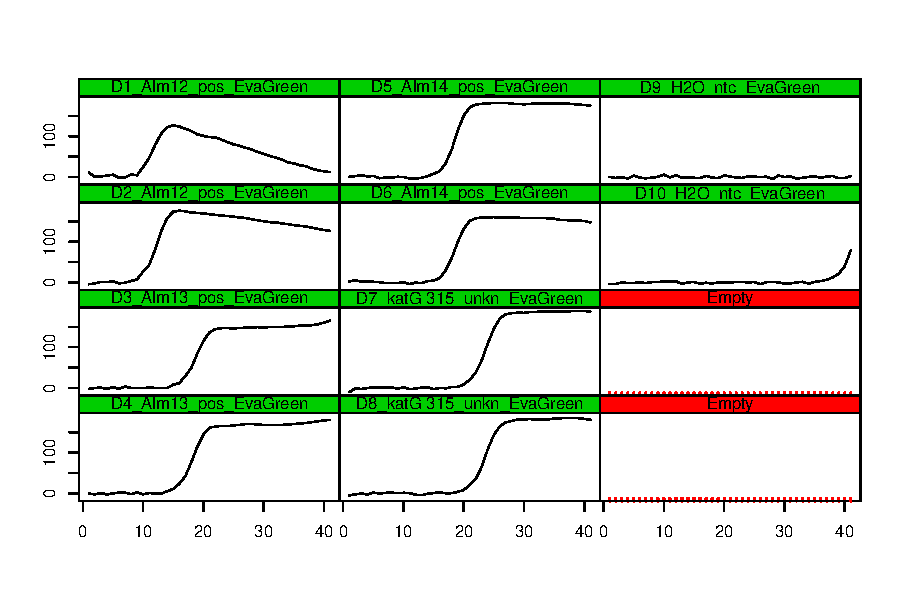
\includegraphics[clip=true,trim=0.1cm 0.6cm 1cm 1.8cm, width=16cm]{figures/plotCurves.pdf}
  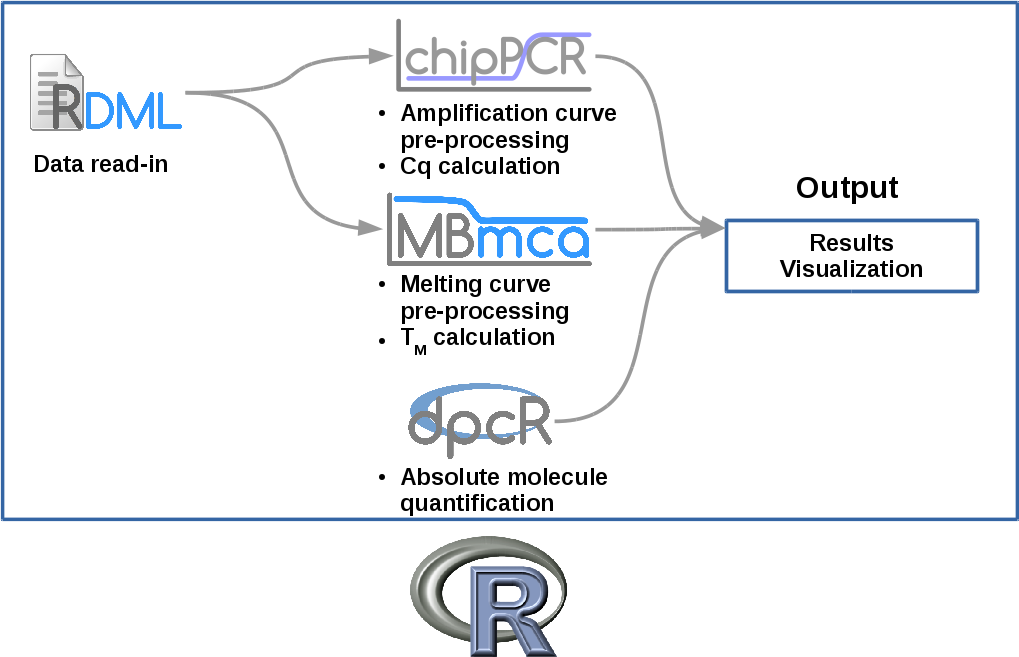
\includegraphics{figures/workflow.png}
  \caption{Exemplary workflow for qPCR experiments in R. Core functionality is 
provided by the R software environment for statistical computing and graphics. 
In our scenario we used the \CRANpkg{RDML} package to read-in data in 
standardized format. However, any format supported by R could be used. Further 
processing of amplification curve data was performed with the \CRANpkg{chipPCR} 
package and amplification curve data were analysed with the \CRANpkg{MBmca} 
package. Cq, quantification cycle; $T_{M}$, melting temperature. The 
\CRANpkg{dpcR} package can be embedded in the analysis 
of digital PCR experiments.
} \label{figure:workflow}
\end{figure}

\section{Setting-up a working environment}

We recommend to perform the scripting in a dedicated integrated development 
environment (IDE) and graphical user interface (GUI) such as \pkg{RKWard} 
\citep{rodiger_rkward_2012}, 
\pkg{Rstudio}\footnote{\url{http://www.rstudio.com/}} or related technologies 
\citep{Valero_2012}. Benefits of IDE's with GUI include syntax-highlighting, 
auto completion and function references for rapid prototyping of workflows.

Typically the qPCR analysis will start with data from a commercial platform. 
Most platforms have an option to export a CSV file or spreadsheets application 
file (e.g., *.xls, *.odt). The details for the import data has been described 
elsewhere \citep{RDCT2010c, rodiger_rkward_2012}. To keep the example sections 
compact we have chosen to load datasets from the \CRANpkg{qcpR} package 
\citep{ritz_2008, spiess_2008} (v.~1.4.0) and \CRANpkg{RDML} package to our 
workspace. In this study we used the \CRANpkg{RDML} package (v.~0.4-2) for data 
read-in. The data were measured with a CFX96 System (Bio-Rad) and then exported 
as RDML v1.1 format file. The \CRANpkg{chipPCR} package (v.~0.0.8-3) was used 
for data preprocessing, quality control and  the calculation of the 
quantification cycle (Cq). The Cq is a quantitative measure, which represents 
the number of cycles needed to reach a user defined threshold fluorescence 
signal level. Typically Cq are determined identically the exponential phase of a 
qPCR reaction. Several Cq methods have been described \citep{ruijter_2013}. In 
this study we have chosen the second derivative maximum method ($Cq_{SDM}$). Due to 
the ubiquitous use we used in a example the ``Cycle threshold'' ($Cq_{Ct}$) method.

In a perfect qPCR reaction, the amount of amplicon doubles ($2^{n}$; n = cycle 
number) at each cycle. Here the amplification efficiency ($AE$) is 100~\%. 
However, in reality, numerous factors cause an inhibition of the amplification 
($AE$ < 100~\%).  The $AE$ can determined be the relation of the Cq value depending 
on the sample input quantity as detailed described in \citep{roediger_chippcr_2014}.

In \citet{roediger_RJ_2013} we described the application of R for the analysis of 
melting curve experiments on the surface of microbeads. Since the mathematical 
foundation for melting curve analysis (MCA) is identical between all platforms 
we applied the functions from the \CRANpkg{MBmca} package 
\citep{roediger_RJ_2013} for an analysis of the target specific melting 
temperature ($T_{M}$) in our qPCR experiment. We used the \CRANpkg{MBmca} 
package (0.0.3-4) for analysis of melting curve data.

We complete our study with a simple example for the analysis of dPCR experiment. 
In particular, we used the \CRANpkg{dpcR} (0.1.3.1) to estimate the number of 
molecules in a sample.

\section{Results}

In this section we will try to show that R is a unified open software which fits 
the needs for (I) data analysis and presentation in research, (II) as software 
frame-work for novel technical developments, (III) as platform for teaching this 
new technology and (IV) serves as reference for statistical methods.

\subsection{Example one -- qPCR and Amplification Efficiency Calculation}

The goal of our fist example was to calculate the Cq values and the $AE$ from a 
qPCR experiment. We used the ``guescini1'' dataset from the \CRANpkg{qcpR} 
package. Details of the experiment are described in \citet{guescini_2008}. A 
good practice for reproducible research is to track the package versions and 
environment used during the analysis. The function $sessionInfo()$ from the 
\CRANpkg{utils} package provides this information. Assuming that the analysis 
starts with a clean R session it is possible to assign the required packages to 
an object only, as shown in our example below\footnote{The reproducibility of 
research can be further improved by using dedicated tools. For example, 
\CRANpkg{archivist} package allows not only stores and recovers crucial data, 
but preserves metadata of saved objects.}.

\begin{example}
# Load the required packages for the data import and analysis.
# Load the chipPCR package for the pre-processing and curve data quality
# analysis.
require(chipPCR)

# Collect information about the R session used for the analysis of the qPCR
# experiment.
current.session <- sessionInfo()

# Next we load the 'guescini1' dataset from the qpcR package the to
# workspace and assign it to the object gue.
require(qpcR)
gue <- guescini1

# Define the diltuion of the sample DNA quantity for
# the calibration curve.

dil <- 10^(2:-4)

# Preprocess the amplification curve data with the CPP function from the chipPCR
# package.
res.CPP <- cbind(gue[, 1], apply(gue[, -1], 2, function(x) {
    CPP(gue[, 1], x, trans = TRUE, method.norm = "minm", bg.range = c(1,7))[["y.norm"]]
}))

# Use the th.cyc function from the chipPCR package to calculate the Cq values
# by the cycle threshold method. The threshold level r was set to 0.05.

Cq.Ct <- apply(gue[, -1], 2, function(x) 
  th.cyc(res.CPP[, 1], x, r = 0.05)[1])
Cq.SDM <- apply(gue[, -1], 2, function(x) 
  summary(inder(res.CPP[, 1], x))[2])

res.Cq <- lm(Cq.Ct ~ Cq.SDM)
\end{example}

\begin{example}
> summary(res.Cq)

Call:
lm(formula = Cq.Ct ~ Cq.SDM)

Residuals:
    Min      1Q  Median      3Q     Max 
-1.4904 -0.2730  0.0601  0.3540  1.1871 

Coefficients:
             Estimate Std. Error t value Pr(>|t|)    
(Intercept) -8.125534   0.207419  -39.17   <2e-16 ***
Cq.SDM       0.988504   0.008097  122.08   <2e-16 ***
---
Signif. codes:  0 ‘***’ 0.001 ‘**’ 0.01 ‘*’ 0.05 ‘.’ 0.1 ‘ ’ 1

Residual standard error: 0.5281 on 82 degrees of freedom
Multiple R-squared:  0.9945,	Adjusted R-squared:  0.9945 
F-statistic: 1.49e+04 on 1 and 82 DF,  p-value: < 2.2e-16
\end{example}

\begin{example}
layout(matrix(c(1,2,3,3,4,5), 3, 2, byrow = TRUE))

matplot(gue[, -1], type = "l", lty = 1, col = 1, xlab = "Cycle", 
	    ylab = "RFU", main = "Raw data")
legend("topleft", "A", cex = 3, bty = "n")

matplot(res.CPP[, -1], type = "l", lty = 1, col = 1, xlab = "Cycle", 
	ylab = "RFU", main = "Pre-processed data")
legend("topleft", "B", cex = 3, bty = "n")
abline(h = 0.05, col = "red", lwd = 2)

plot(Cq.SDM, Cq.Ct, xlab = "Ct method", ylab = "SDM method", 
     main = "Comparison of Cq methods")
abline(res.Cq)
legend("topleft", "C", cex = 3, bty = "n")

plot(effcalc(dil, t(matrix(Cq.Ct, nrow = 12, ncol = 7))), CI = TRUE)
legend("topright", "D", cex = 3, bty = "n")

plot(effcalc(dil, t(matrix(Cq.SDM, nrow = 12, ncol = 7))), CI = TRUE)
legend("topright", "E", cex = 3, bty = "n")
\end{example}

\begin{figure}[htbp]
  \centering
%   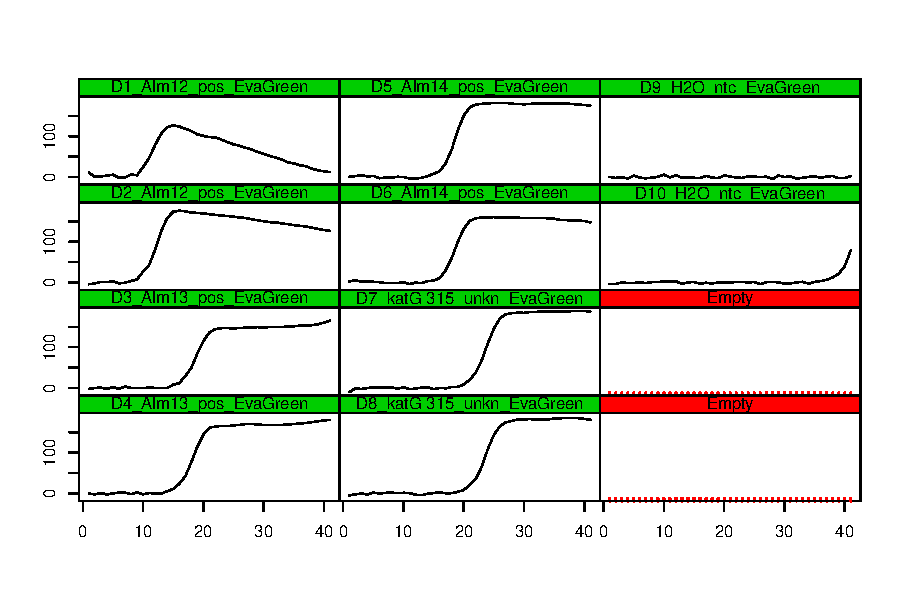
\includegraphics[clip=true,trim=0.1cm 0.6cm 1cm 1.8cm, width=16cm]{figures/plotCurves.pdf}
  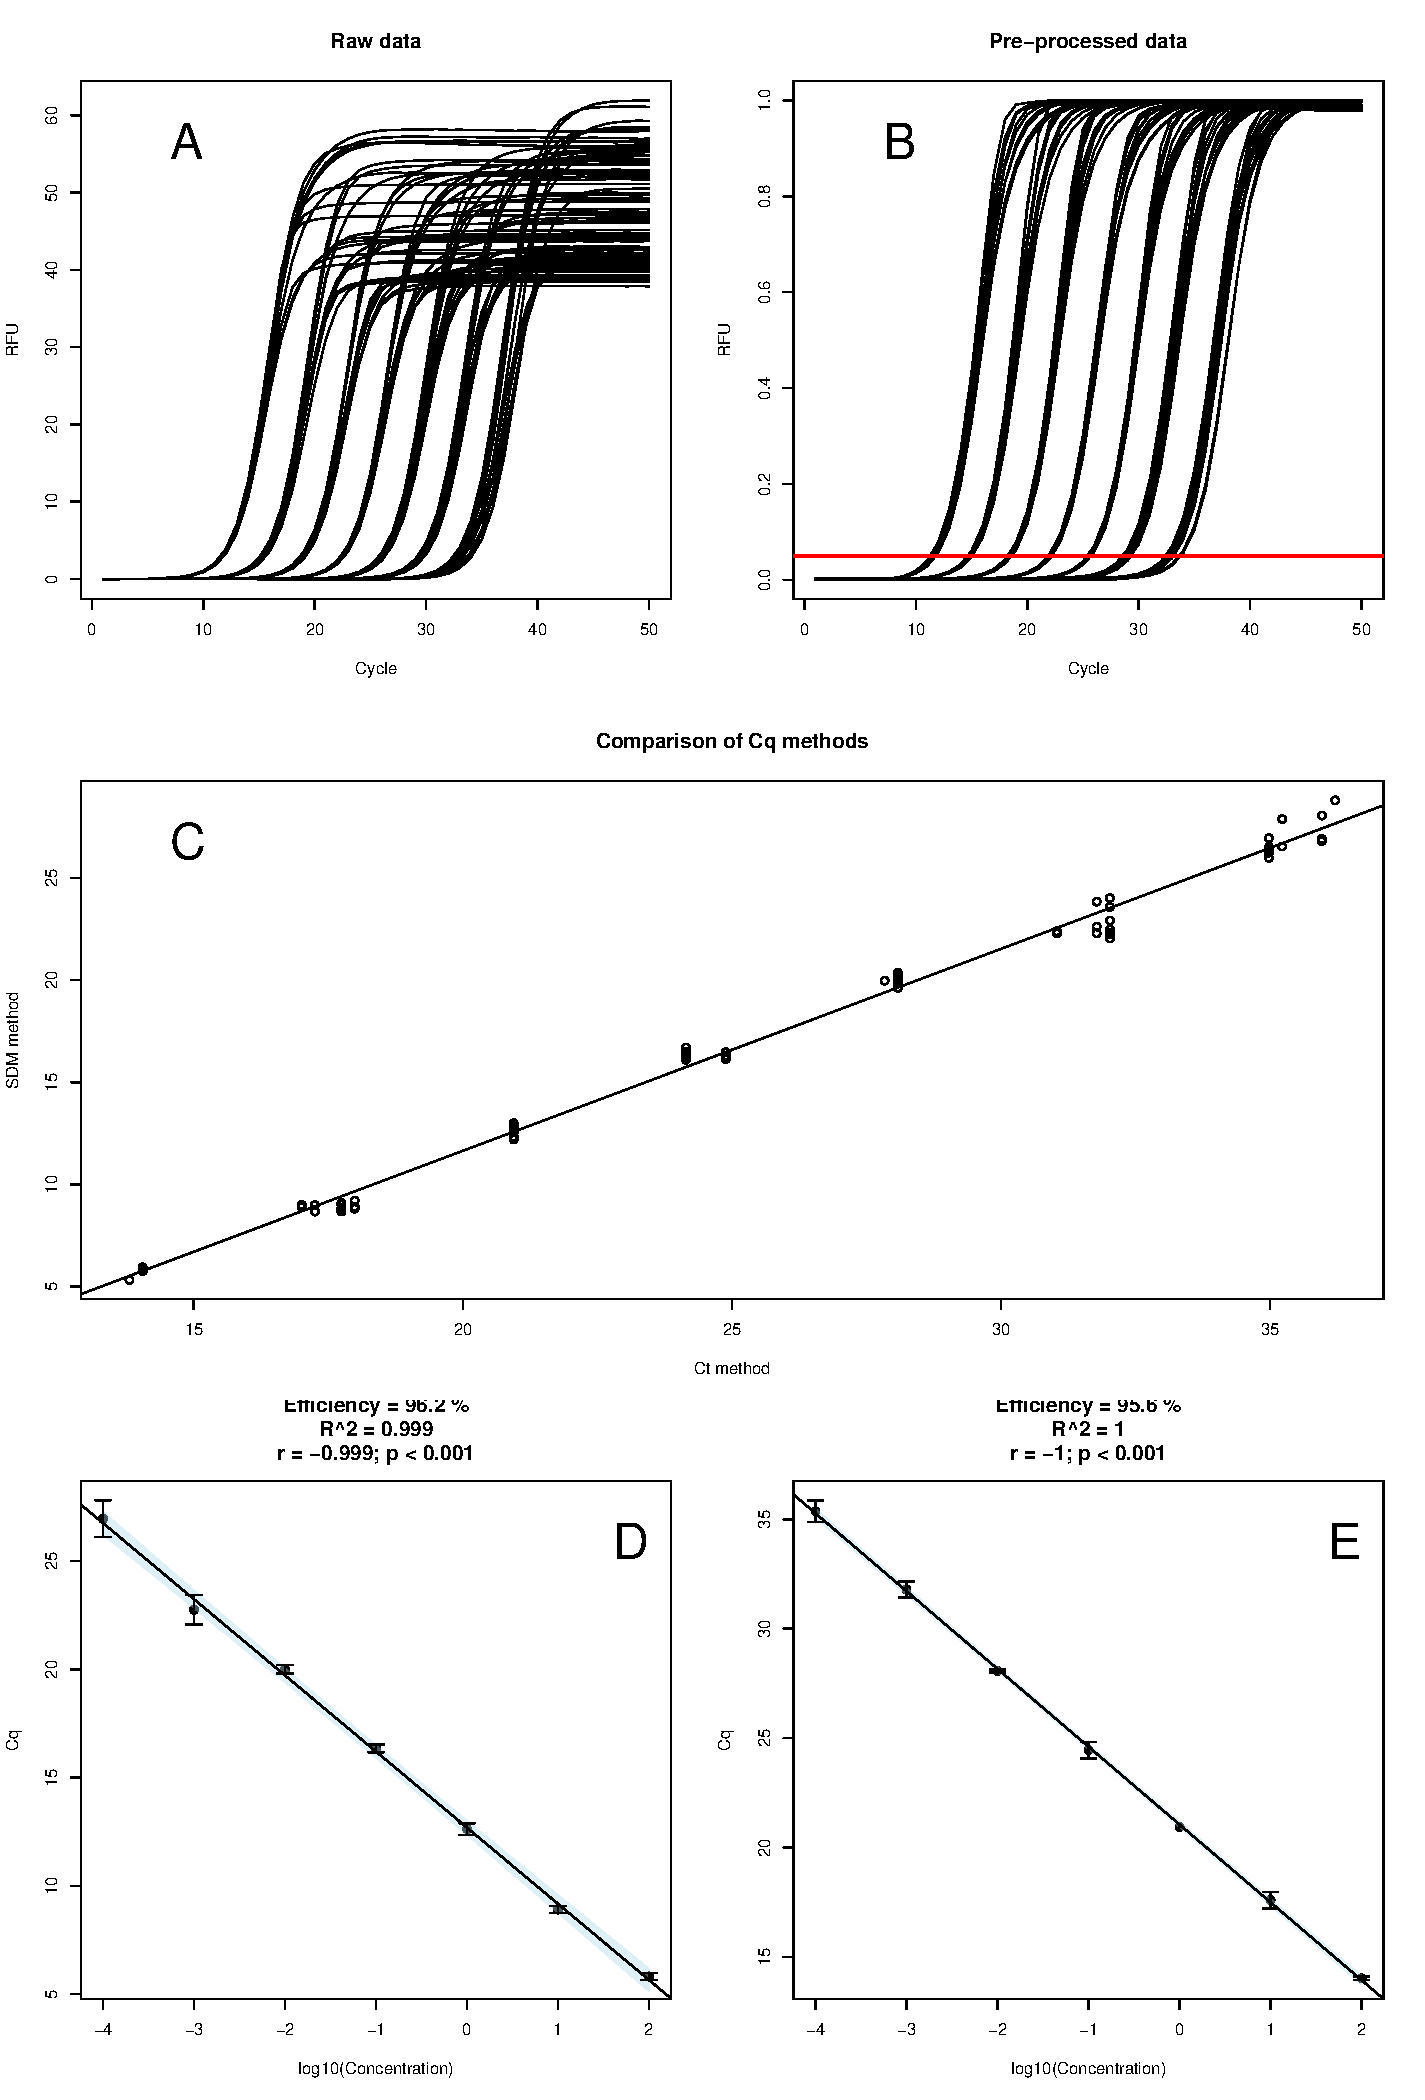
\includegraphics[clip=true, width=14cm]{figures/dilution_Cq.pdf}
  \caption{Analysis of the amplification curve data of the calibration curve 
samples. \strong{(A)} Visual inspection of the raw data from the \texttt{guescini1} 
dataset. The qPCR curves display a broad variation in plateau fluorescence (38 
-- 62 RFU). The red horizontal line indicates the fluorescence level (0.05) used 
for the calculation of the Cq by the ``cycle threshold'' method. \strong{(B)} 
the \code{CPP} function from the \CRANpkg{chipPCR} was sued to baseline the 
data, to smooth the data with Savitzky-Golay smoothing filter and to normalize 
the data between 0 and 1. \strong{(C)} The Cq values were calculated for the 
second derivative maximum ($Cq_{SDM}$) method (\code{inder}, \CRANpkg{chipPCR}) 
and the cycle threshold method ($Cq_{Ct}$) (\code{th.cyc}, \CRANpkg{chipPCR}). 
The threshold value was set to $r~=~0.05$. The $Cq_{SDM}$ and $Cq_{Ct}$ values 
were plotted and analysed by a linear regression ($R^{2}~=~0.9945$; $P < 
2.2^{-16}$) and Pearson's ($r~=~0.9972605$; $P < 2.2^{-16}$). The $AE$ based on 
\strong{(D)} $Cq_{Ct}$ values and \strong{(E)} $Cq_{SDM}$ values were 
automatically analysed with the \code{effcalc} (\CRANpkg{chipPCR}) function.}
  \label{figure:dilution_Cq}
\end{figure}

\subsection{Example two -- qPCR and Melting Curve Analysis}

A common task during the analysis of qPCR experiments is to distinguish between 
positive and negative samples (compare Figure~\ref{figure:plotCurves}). Provided 
that the melting temperature of a sample is known it is possible to automatize 
the melting curve analysis (MCA). As shown in \citet{roediger_RJ_2013} this can 
be done by interrogating the $T_{M}$. Therefore, we used a simple logic statement, 
which checks if $T_{M}$ is within a tight temperature range and signal height. In line 
with ``Example one'' we used function $sessionInfo()$ to track the packages used 
for the analysis. Reproducible research is greatly enhanced of open data 
exchange formats are used. In this study we used the \CRANpkg{RDML} package to 
read the qPCR experiment. The example file \file{BioRad\_qPCR\_melt.rdml} for 
analysis was taken from the \CRANpkg{RDML} package. Within this qPCR experiment 
we amplified the \textit{Mycobacterium tuberculosis} 
\textit{katG}\footnote{\url{https://www.wikigenes.org/e/gene/e/923602.html}} 
gene to detect mutation at codon 315. The experiment was separated for two parts: 
(I) detection of overall \textit{M.tuberculosis} DNA (wild-type and mutant) by 
intercalating dye EvaGreen® within qPCR and (II) specific detection of wild-type 
\textit{M.tuberculosis} by melting of TaqMan probe (quencher -- BHQ2, 
fluorescent reporter -- Cy5) with amplified DNA (similar assay is described in 
\citet{luo_multiplex_2011}). Real time amplification were conducted using Syntol 
EvaGreen Master Mix according to the manufacturer's instructions, with 500 nM of 
primers and probe in a 25 $\mu$L final reaction volume. Thermocycling was 
conducted using a CFX96 (BioRad) initiated by 3 min incubation at 
95~\textcelsius, followed by 41 cycles (15 s at 95~\textcelsius; 40 s at 
65~\textcelsius) with a single fluorescent reading taken at the end of each 
cycle. Probe melting was conducted between 35~\textcelsius~and 
95~\textcelsius~by 1~\textcelsius at 1 s steps.
\begin{example}
# Load the required packages for the data import and analysis.

# Import the qPCR and melting curve data via the RDML package
require(RDML)

# Load the chipPCR package for the pre-processing and curve data quality
# analysis.
require(chipPCR)

# Load the MBmca package for the melting curve analysis.
require(MBmca)

# Collect information about the R session used for the analysis of the qPCR
# experiment.
current.session <- sessionInfo()


# Load the BioRad_qPCR_melt.rdml file form RDML package and assign the data to the
# object BioRad.

filename <- paste(path.package("RDML"), "/extdata/", "BioRad_qPCR_melt.rdml", sep = "")
BioRad <- RDML(filename, name.pattern = "%TUBE%_%NAME%_%TYPE%_%TARGET%")

# Fetch cycle dependent fluorescence for the EvaGreen channel of the 
# Mycobacterium tuberculosis katG gene and aggregate the data in the 
# object qPCR. 
qPCR <- cbind(BioRad[["qPCR"]][["EvaGreen"]][["pos"]], 
	      BioRad[["qPCR"]][["EvaGreen"]][["unkn"]][, -1], 
	      BioRad[["qPCR"]][["EvaGreen"]][["ntc"]][, -1])
# Leave data only from row 'D' that contains target 'Cy5-2' at channel 'Cy5'
qPCR <- cbind(qPCR[,1], qPCR[, grep("^D", names(qPCR))])
\end{example}

We inspected and pre-processed a subset of the amplification curve data 
solely using functionalities provided by the \CRANpkg{chipPCR} package. The 
\code{plotCurves} function was used to get an overview of the curvatures. The 
data indicated a baseline shift in all curves with a slight negative trend 
(Figure~\ref{figure:plotCurves}). This suggested to baseline the raw data by 
using a linear regression model (cycles x - y; ($bg.range = c(x, y)$) in the 
\code{CPP} function.).

\begin{example}
# Use plotCurves function from the chipPCR package to get an overview of the
# amplification curve samples.

plotCurves(qPCR[, 1], qPCR[, -1], type = "l")

# Detect positive samples - calculate Cq values
# by the cycle threshold method. The threshold level r was set to 50.
Cq.Positive <- t(apply(qPCR[, -1], 2, function(x)
{
  res <- CPP(qPCR[, 1], x, trans = TRUE, bg.range = c(2, 8))[["y.norm"]]
  th.cyc <- th.cyc(qPCR[, 1], res, r = 50)[1]
  cq <- as.numeric(th.cyc)
  pos <- !is.na(cq)
  c(Cq=cq, M.Tub_positive = pos)
}
))
Cq.Positive
\end{example}

Since the qPCR indicated that selected samples (except no template control) are positive, we started to 
distinguish between true positive and true negative samples by MCA.
\begin{example}
# Fetch temperature dependent fluorescence for the Cy5 channel of the 
# probe that can hybridize with Mycobacterium tuberculosis katG gene (codon 315)
# and aggregate the data in the object melt.
melt <- cbind(BioRad[["Melt"]][["Cy5-2"]][["pos"]],
              BioRad[["Melt"]][["Cy5-2"]][["unkn"]][, -1],
              BioRad[["Melt"]][["Cy5-2"]][["ntc"]][, -1])

# Calculate the melting temperature with the diffQ function
# from the MBmca package. Use simple logical conditions to find out
# if a positive sample with the expected Tm of circa 54.5 degree 
# Celsius is found.
Tm.Positive <- matrix(nrow = length(melt[, -1]),
                      byrow = TRUE,
                      dimnames = list(names(melt)[-1]),
                      unlist(apply(melt[, -1], 2, function(x) {
  res.Tm <- diffQ(cbind(melt[, 1], x), fct = max, inder = TRUE)
  positive <- ifelse(res.Tm[1] > 54 & res.Tm[1] < 55 & res.Tm[2] > 80, 1, 0)
  c(res.Tm[1], res.Tm[2], positive)
})))

# Present the results in a tabular output as data.frame "results.tab".
# Result of analysis logic is:
# Cq.Positive && Tm.Positive = Wild-type
# Cq.Positive && !Tm.Positive = Mutant
# !Cq.Positive && !Tm.Positive = NTC
# !Cq.Positive && Tm.Positive = Error
results <- sapply(1:length(Cq.Positive[,1]), function(i) {
  if(Cq.Positive[i, 2] == 1 && Tm.Positive[i, 3] == 1)
    return("Wild-type")
  if(Cq.Positive[i, 2] == 1 && Tm.Positive[i, 3] == 0)
    return("Mutant")
  if(Cq.Positive[i, 2] == 0 && Tm.Positive[i, 3] == 0)
    return("NTC")
  if(Cq.Positive[i, 2] == 0 && Tm.Positive[i, 3] == 1)
    return("Error")
})
results.tab <- data.frame(cbind(Cq.Positive, Tm.Positive, results))
names(results.tab) <- c("Cq", "M.Tub DNA", "Tm", "Height", "Tm positive", "Result") 
results.tab[["M.Tub DNA"]] <- factor(results.tab[["M.Tub DNA"]], labels=c("Not Detected",
                                                                  "Detected"))
results.tab[["Tm positive"]] <- factor(results.tab[["Tm positive"]], labels=c(TRUE,
                                                                  FALSE))
results.tab
\end{example}

Finally, we plotted and printed the output of our analysis.

\begin{example}
# Convert the Decission from the "relsults" object in a color code:
# Negative, black; Positive, red.

color <- c(Tm.Positive[, 3] + 1)

# Arrange the results of the calculations in plot.
layout(matrix(c(1,2,1,3), 2, 2, byrow = TRUE))

# Use the CPP function to preporcess the amplification curve data.
plot(NA, NA, xlim = c(1, 41), ylim = c(0,200), xlab = "Cycle", ylab = "RFU")
mtext("A", cex = 2, side = 3, adj = 0, font = 2)
lapply(2L:ncol(qPCR), function(i) 
  lines(qPCR[, 1], 
        CPP(qPCR[, 1], qPCR[, i], trans = TRUE, 
            bg.range = c(1,9))[["y.norm"]],
        col = color[i - 1]))
matplot(melt[, 1], melt[, -1], type = "l", col = color, 
	lty = 1, xlab = "Temperature [°C]", ylab = "RFU")
mtext("B", cex = 2, side = 3, adj = 0, font = 2)
	
plot(NA, NA, xlim = c(35, 95), ylim = c(-15, 120), xlab = "Temperature [°C]", 
     ylab = "-d(RFU)/dT")
mtext("C", cex = 2, side = 3, adj = 0, font = 2)
lapply(2L:ncol(melt), function(i)
  lines(diffQ(cbind(melt[, 1], melt[, i]), verbose = TRUE, 
              fct = max, inder = TRUE)[["xy"]], col = color[i - 1]))
              
\end{example}


\begin{figure}[htbp]
  \centering
  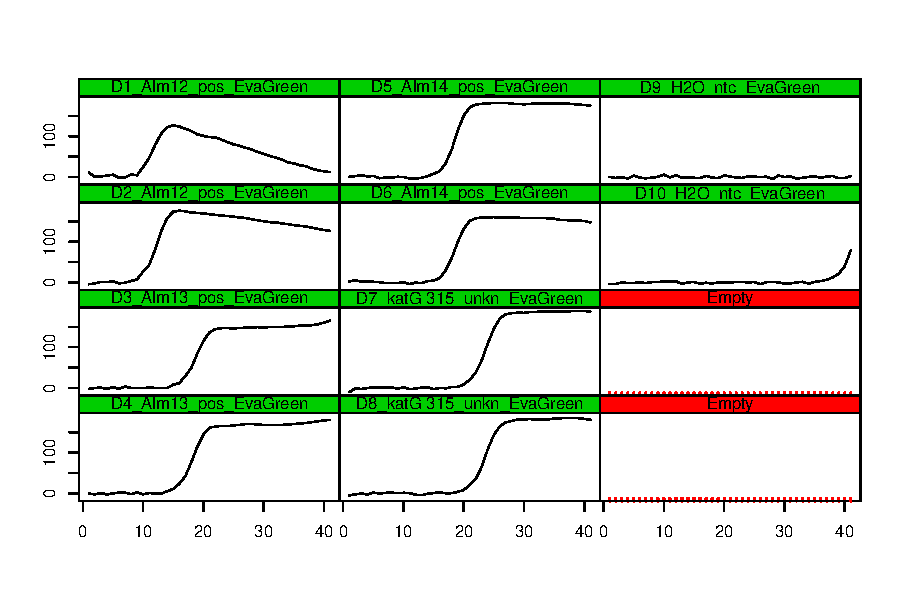
\includegraphics{figures/plotCurves.pdf}
  \caption{Analysis of the amplification curve data of the calibration curve 
samples by the \code{plotCurves} function from the \CRANpkg{chipPCR} package. 
The green color code indicates that the data contains no missing values. 
However, the visual inspection revealed that the data are noisy. All samples 
(``D1\_Alm12\ldots'' - ``D8\_Alm12\ldots'') appeared to be positive. One 
negative control (``D10\_H20\_ntc\_EvaGreen'') appeared to be contaminated.}
  \label{figure:plotCurves}
\end{figure}

\begin{figure}[htbp]
  \centering
  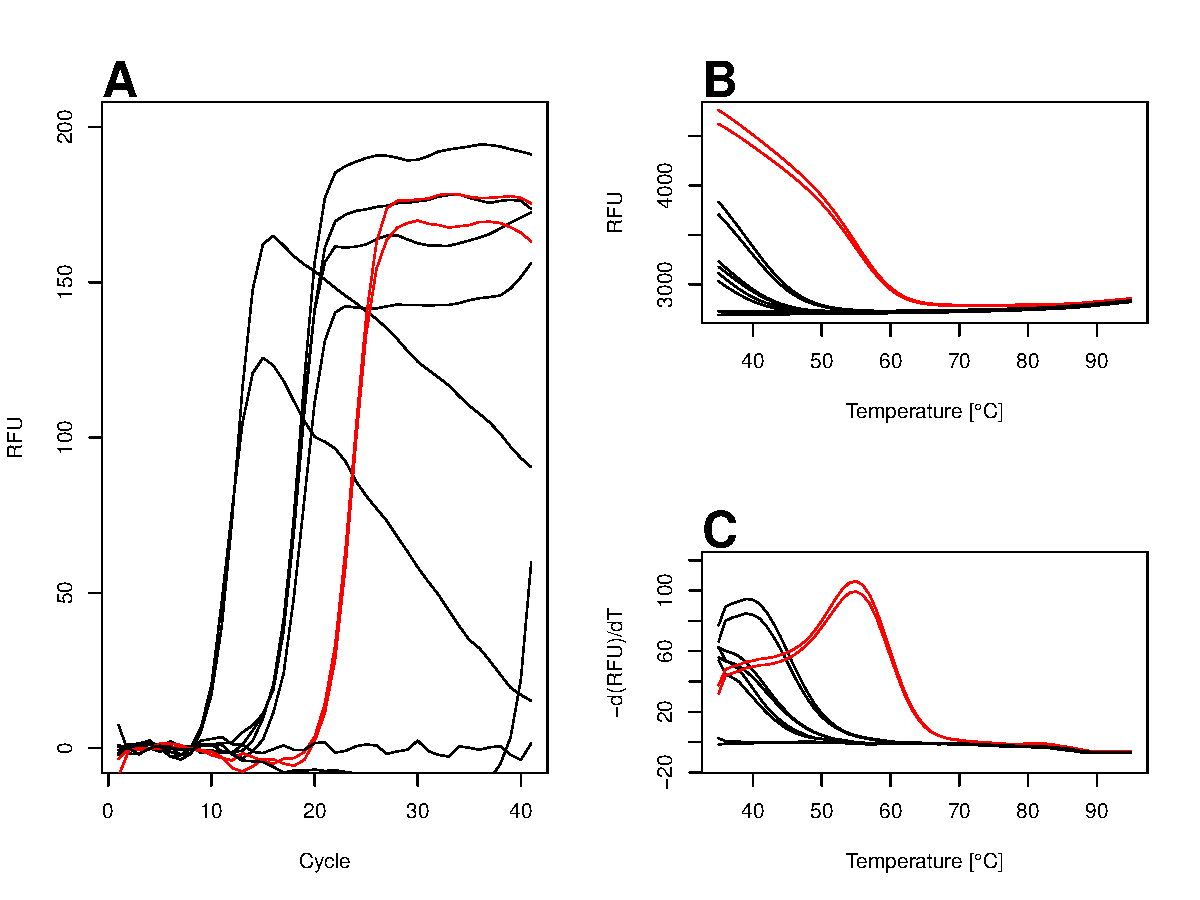
\includegraphics[clip=true, width=16cm]{figures/amp_melt.pdf}
  \caption{Graphical presentation of the amplification curve data and melting 
curve data. \strong{(A)} The raw amplification curve data were pre-process with 
the \code{CPP} function prior to visualization. To calculate the $T_{M}$ values 
from the raw melting curve data \strong{(B)} we used the \code{diffQ} function 
from the \CRANpkg{MBmca} package. \strong{(C)} In our setting we adjusted the algorithm to 
plot the positive melting peaks in red, while negative melting peaks were 
labelled in black.} 
\label{figure:amp_melt}
\end{figure}

\subsection{Example three -- Isothermal Amplification}

Isothermal amplification is an alternative to PCR \citep{rodiger_nucleic_2014}. 
In contrast to PCR use isothermal amplification methods a constant temperature 
rather than cycling through denaturation, annealing and extension steps. The 
corresponding signal is monitored depending on the time instead of cycles. We 
performed a quantitative isothermal amplification (qIA) for the target 
\textit{pCNG1}\footnote{The HDA conditions were taken from the ``IsoAmp III 
Universal tHDA Kit'', Biohelix Corp, as described by the vendor. In detail, the 
reaction was composed of ``mix A)'' 10 $\mu$L A. bidest, 1.25 $\mu$L 10xb~uffer, 
0.75 $\mu$L primer(150 nM final), 0.5 $\mu$L template plasmid. Preincubation: 
The mixture was incubated for 2 min at 95\textcelsius and immediately placed on 
ice. Reaction ``mix B)'' contained 5 $\mu$L A. bidest., 1.25 $\mu$L 10x buffer, 
2 $\mu$L NaCl, 1.25 $\mu$L MgSO_{4}, 1,75 $\mu$L dNTPs, 0.25 $\mu$L EvaGreen 
(Biotium), 1 $\mu$L enzyme mix. The mix was covered with 50 $\mu$L mineral oil 
(Roth). The fluorescence measurement in VideoScan HCU started directly after 
adding ``mix B)'' at 65\textcelsius. A $1x$ (D1) and a $1:10$ dilution (D2) were 
tested.} by using a Helicase Dependent Amplification (HDA). The enzyme DNA 
Helicase unwinds DNA. Therefore, no thermal denaturation is needed. Our 
previously reported VideoScan platform \citep{rodiger_highly_2013} was used 
to measure the samples. The resulting dataset \texttt{C81} is part of the 
\CRANpkg{chipPCR} package. Two concentrations (stock and 1:10 diluted stock) of 
input DNA were used in the HDA.

\begin{example}
# Drawn in an 2-by-1 array on the device by two columns and one row.
par(mfrow = c(2, 1))

# Plot the raw data from the C81 dataset to the first array and add
# a legend.
plot(NA, NA, xlim = c(0, 120), ylim = c(0.4, 1.2), xlab = "Time (min)", ylab = "RFU")
mtext("A", cex = 2, side = 3, adj = 0, font = 2)
lapply(c(2, 4), function(i) {
    lines(C81[, i]/60, C81[, i + 1], type = "b", pch = 20, col = i - 1)
})
legend(10, 0.8, c("D1: 1x", "D2: 1:10 diluted sample"), pch = 19, col = c(1, 3), 
    bty = "n")
\end{example}

\begin{example}
# Prepare a plot on the second array for the pre-proccessed data.
plot(NA, NA, xlim = c(0, 120), ylim = c(0, 0.8), xlab = "Time (min)", ylab = "RFU")
mtext("B", cex = 2, side = 3, adj = 0, font = 2)

# Apply the CPP functions to pro-process the raw data.
# 1) Baseline data to zero, 2) Smooth data with spline,
# 3) Remove outliers in background range between 
# entry 1 and 190.
res <- lapply(c(2, 4), function(i) {
  y.s <- CPP(C81[, i]/60, C81[, i + 1],
             trans = TRUE, 
             method = "spline",
             bg.outliers = TRUE,
             bg.range = c(1, 190))
  lines(C81[, i]/60, y.s[["y.norm"]], type = "b", pch = 20, col = i - 1)
  # Use the th.cyc function to calculate the cycle threshold time. 
  # The threshold level r was set to 0.05.
  paste(round(th.cyc(C81[, i]/60, y.s[["y.norm"]], r = 0.05)[1], 2), "min")
})

# Add the cycle threshold time and the threshold level to plot.

abline(h = 0.05, lty = 2)
text(10, 0.55, "Cq:")
legend(10, 0.5, paste(c("D1: ", "D2: "), res), pch = 19, col = c(1, 3), bty = "n")
\end{example}



\begin{figure}[htbp]
  \centering
  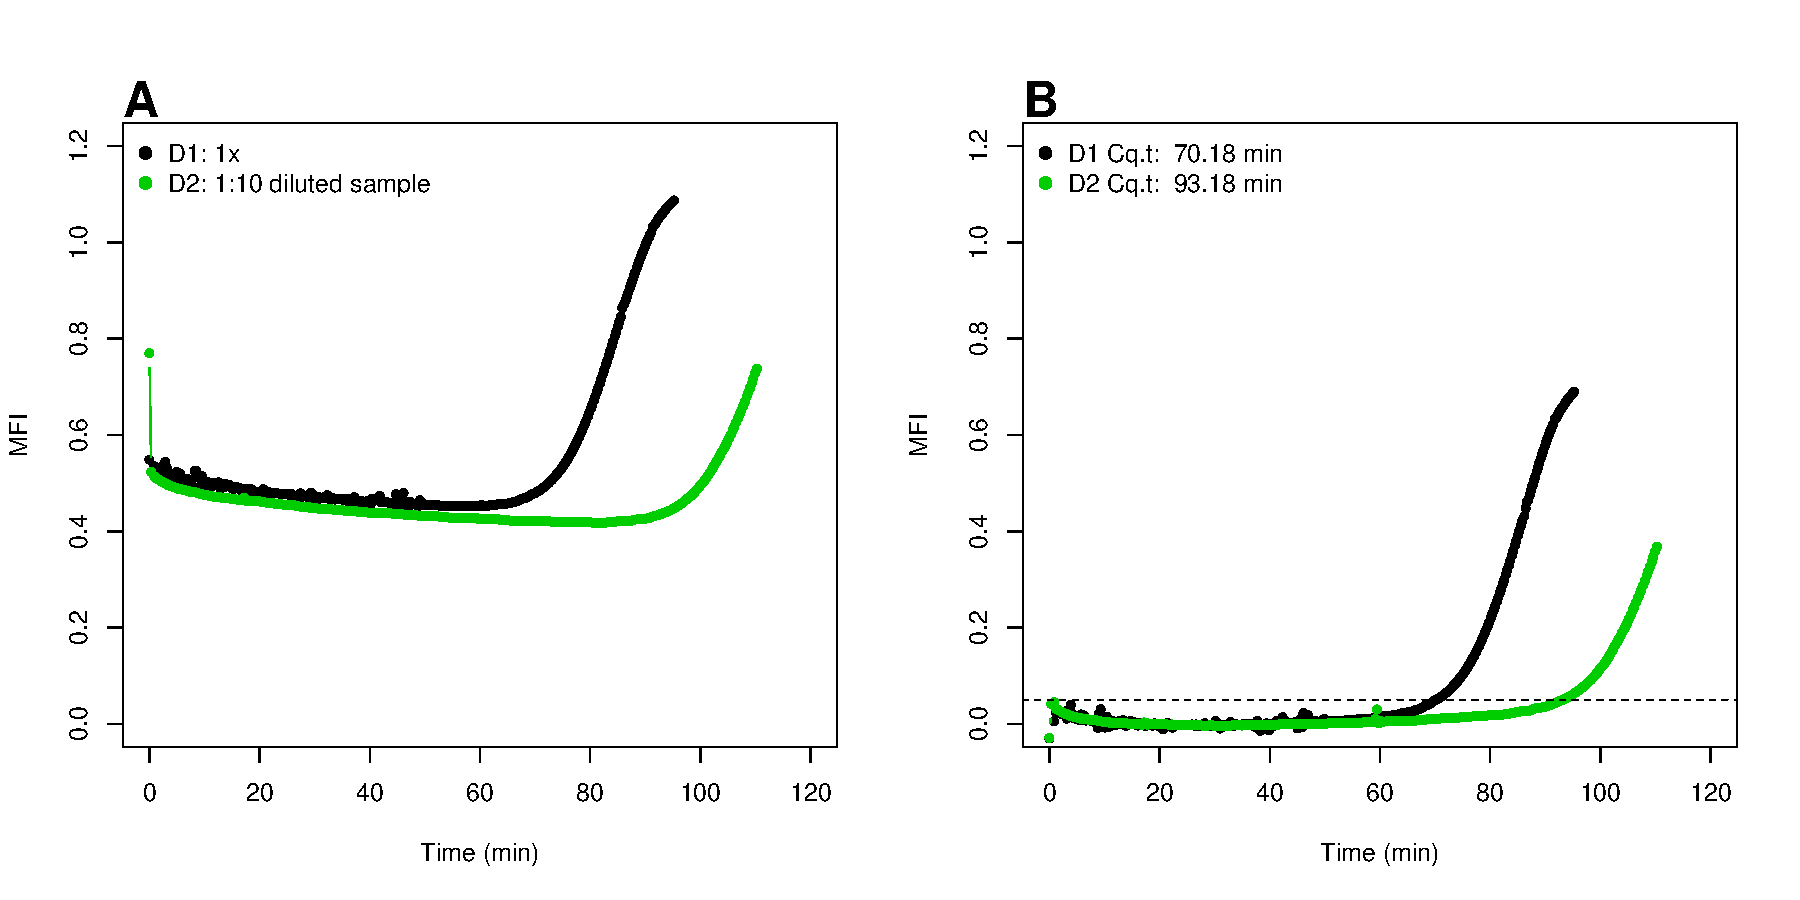
\includegraphics[clip=true, width=16cm]{figures/qIA.pdf}
  \caption{Quantitative isothermal amplification by Helicase Dependent 
Amplification (HDA). \strong{(A)} The raw data of the HDA (D1, undiluted, D2 
$1:10$ diluted) exhibit some outliers (detector artifacts), an off-set of circa 
0.5 relative fluorescence units (RFU) and a slight negative trend in the 
baseline region (0 to ~52 minutes). \strong{(B)} First we used the \code{CPP} 
function from the \CRANpkg{chipPCR} package to smooth the data with spline 
function. Baselining was done with a robust MM-estimator (range 0 to 52 min). 
Finally, we used the \code{th.cyc} function from the \CRANpkg{chipPCR} package 
to calculate the cycle threshold time for samples D1 and D2. The threshold value 
was set to $r = 0.05$ ($--$).}
  \label{figure:qIA}
\end{figure}

\subsection{Example four - digital PCR}

We have developed the \CRANpkg{dpcR} package for analysis and presentation of 
digital PCR experiments. The \CRANpkg{dpcR} package can be used to build 
custom-made analysers and provides structures to be openly extended by the 
scientific community. Simulations and predictions of binomial and Poisson 
distributions, commonly used theoretical models of dPCR, statistical data 
analysis methods, plotting facilities and report generation tools are part of 
the package \citep{pabinger_2014}. Here, we show briefly an example for the 
\CRANpkg{dpcR}. Figure~\ref{figure:dpcR_sim}.

In detail, we mimicked an in-silico experiment for a droplet digital PCR. The aim was to do a density 
estimation. The number of positive partitions ($k$), total number of partitions ($n$) and 
the size of the partition are only data required for analysis. The estimate of 
the mean number of template molecules per partition ($\hat \lambda$) is 
calculated using following equation \citep{huggett_2013}:

\begin{equation}
\hat{\lambda} =  -\ln{(1 - \frac{k}{n})}.
\end{equation}

The average droplet value in our experiment was assumed to be 5 nL. We counted 
$n$ = 16800 droplets in total and $k$ = 4601 droplets were positive. Since the 
binomial distribution of positive and negative partitions is used to define 
$\lambda$, we use Wilson method for calculation of confidence intervals 
\citep{brown_2001}. The obtained mean number of template molecules per partition 
multiplied by the volume of the partitions constitutes concentration of a 
template in the sample.

\begin{example}
# Load the dpcR package for the analysis of the digital PCR experiment.
require(dpcR)

# In our in-silica experiment we counted in total 16800 droplets (n). 
# Thereof, 4601 were positive (k).

(dens <- dpcr_density(k = 4601, n = 16800, average = TRUE, methods = "wilson"))

# Let us assume, that every droplet has roughly 5 nL 
# total concentration (and its confidence intervals) in molecules/mL
dens[4:6] / 5 * 1e-6
#results: 
#concentration        lower       upper
#6.400498e-08  6.217049e-08 6.58852e-08
\end{example}

Selected functionality was implemented as interactive \CRANpkg{shiny} GUI 
application to make the software accessible for users who are not fluent in R 
and for experts who wish to automatize routine tasks. Details and examples of 
the \CRANpkg{shiny} web application framework for R can be found at 
\url{http://shiny.rstudio.com/}. We implemented flexible yet simple user 
interfaces, which run the analyses and graphical representation into interactive 
web applications either as service on a web severer or on a local machine 
without knowledge of HTML or ECMAScript (see \CRANpkg{dpcR} manual). The 
interface is designed in a cascade workflow approach (Data import $\rightarrow$ 
Analysis $\rightarrow$ Output $\rightarrow$ Export) with interactive users 
choice on input data, methods and parameters using typical GUI elements such as 
sliders, drop-downs and text fields. An example can be found at 
\url{https://michbur.shinyapps.io/dpcr_density/}. This approach enables the 
automatized outputs of R objects in combined plots, tables and summaries.

\begin{figure}[htbp]
  \centering
  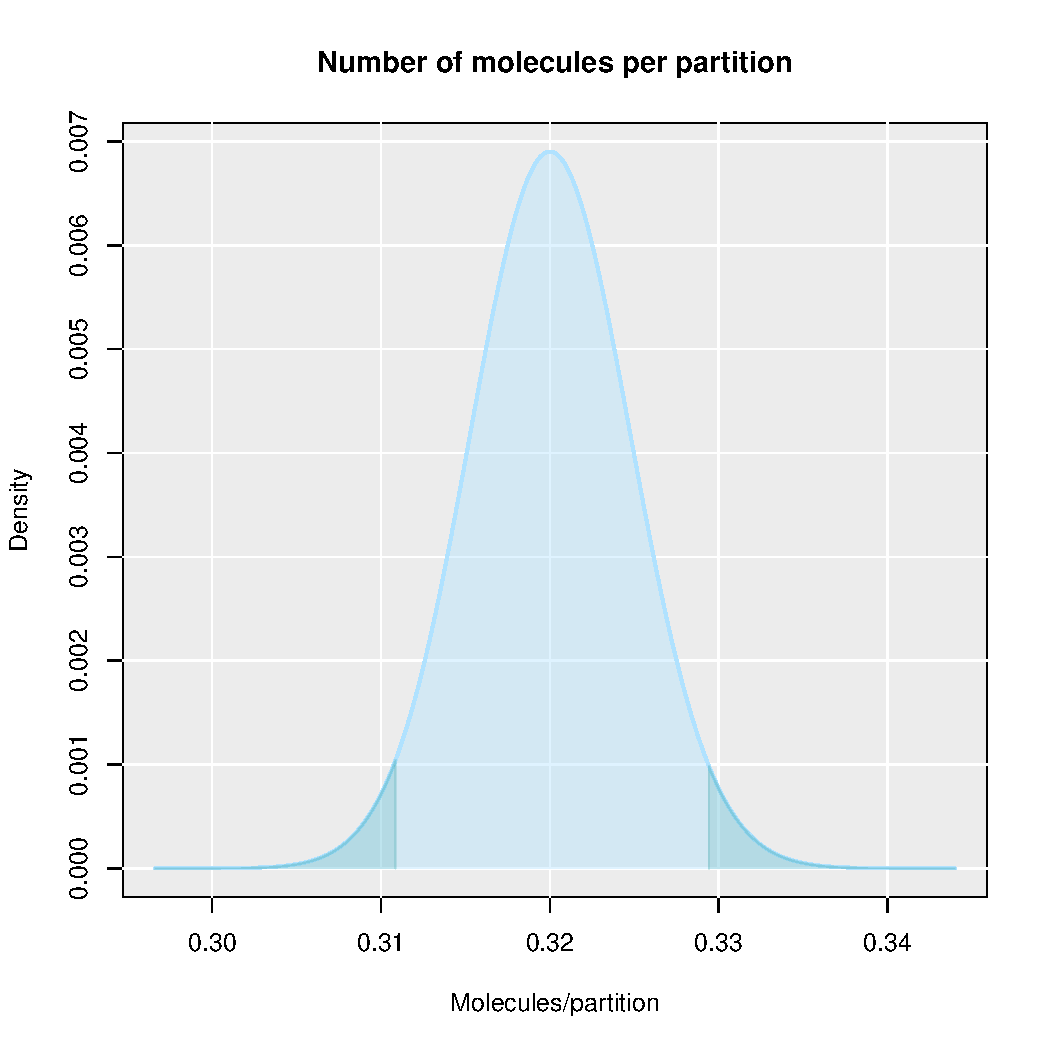
\includegraphics[clip=true, width=14cm]{figures/dpcR.pdf}
  \caption{\code{dpcr\_density} function from the \CRANpkg{dpcR} package used 
for analysis of droplet digital PCR experiment. From 16800 counted droplets 
($n$) 4601 were positive ($k$). Estimated mean number of template molecules per 
partition ($\lambda$) is 0.32.
}
  \label{figure:dpcR}
\end{figure}

\section{Discussion and Conclusion}

This study gave a brief introduction how to perform a qPCR, qIA or dPCR analysis 
with R based on packages available from CRAN. In addition, we briefly referenced 
to a vast collection of additional packages available from CRAN and 
Bioconductor. The packages may be considered building blocks (libraries) to 
create what users want and need. We showed that automatized research with R 
offers powerful means for statistical analysis and visualization. The software 
is not tied to a vendor or specific application (e.g., chamber or droplet based 
digital PCR, capillary or plate qPCR). It should be quite easy even for an 
inexperienced user to define a workflow and to set up environment for specific 
needs in a broad range of technical settings (Figure~\ref{figure:options}). R 
enforces no monolithic integration. We claim that the modular structure of R 
packages allows user to perform flexible data analysis adjusted to their needs 
and to design frameworks for high-throughput analysis. R allows to access and 
reuse code for the creation of reports in various formats (e.g., HTML, PDF). 
Most of the software is cross-platform open source software and is freely 
available from CRAN or Bioconductor. Despite the fact that R is free of charge 
it is quite possible to build commercial applications. The packages cover 
implementation of novel approaches and peer-reviewed analysis methods. R 
packages are an open environment to adopt to the growing knowledge in dPCR and 
qPCR. Therefore, we argue that R may provide a structure for standardized 
nomenclature and serve as reference in qPCR and dPCR analysis. Speaking about 
openness, it is important to emphasize that main advantage is the software is 
transparent at any time for anybody. Thus, it is possible to track numerical 
errors.  A serve disadvantage of R is the lack of comprehensive GUIs for qPCR 
analysis. Other and we believe that a graphical user interface (GUI) is a key 
technology to spread the use of R in bioanalytical sciences. Currently, we are 
establishing the ``pcRuniveRsum'' (\url{http://michbur.github.io/pcRuniveRsum/}) 
as an on-line resource for interested users. The command-line structure makes R 
``inaccessible'' for many novices. This we support the attempt that automatic 
routines are made accessible via GUIs \citep{rodiger_rkward_2012}. However, work 
in this has recently started and is still under development.

\begin{figure}[htbp]
  \centering
  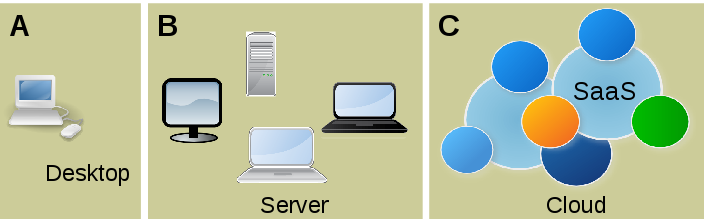
\includegraphics[clip=true, width=10cm]{figures/options.png}
  \caption{Deployment of R applications for the qPCR and dPCR experiments. 
\strong{(A)} R is typically run from a desktop computer an operated by an 
GUI/IDE application such as \pkg{Rstudio} or \pkg{RKWard}. This approach is 
provides a flexible workflow for individuals. \strong{(B)} Another approach is 
to run R with specific applications on a local server. Such scenarios are useful 
for the deployment within research departments or cooperate units. \strong{(C)} 
Cloud computing (CC) provides shared and scalable computing capacity (e.g., 
computing capacity, application software) and storage capacity (e.g., databases) 
as a service to an individual user or a community Service categories include: 
Infrastructure-as-a-Service (IaaS), Platform-as-a-Service (PaaS) and 
Software-as-a-Service (SaaS) over a network. Providers of CC manage the 
infrastructure and resources to achieve coherence and economies of scale similar 
to a utility over a network (typically the Internet).}
  \label{figure:options}
\end{figure} 

\section{Acknowledgment}

Part of this work was funded by the BMBF InnoProfile-Transfer-Projekt 03 IPT 
611X. We would like to thank R community. Part of this work was funded by the 
Russian Ministry of Education and Science (project No. RFMEFI62114X0003) and 
with usage of scientific equipment of Center for collective use 
``Biotechnology'' at All-Russia Research Institute of Agricultural 
Biotechnology. We would like to thank Mario Menschikowski (Technical University 
Dresden) for the droplet digital PCR samples.

\bibliography{Roediger_2014_R}

\address{Stefan R\"odiger (corresponding author)\\
  Faculty of Natural Sciences\\
  Brandenburg University of Technology Cottbus--Senftenberg\\
  Senftenberg\\
  Germany}
\email{Stefan.Roediger@hs-lausitz.de}

\address{Micha\l{} Burdukiewicz\\
  University of Wroclaw\\
  Faculty of Biotechnoloy\\
  Department of Genomics\\
  Wroclaw\\
  Poland}
\email{michalburdukiewicz@gmail.com}

\address{Konstantin Blagodatskikh\\
  All-Russia Research Institute of Agricultural Biotechnology\\
  Center for collective use ``Biotechnology''\\
  Moscow\\
  Russia}
\email{k.blag@yandex.ru}

\address{Peter Schierack\\
  Faculty of Natural Sciences\\
  Brandenburg University of Technology Cottbus--Senftenberg\\
  Senftenberg\\
  Germany}
\email{Peter.Schierack@hs-lausitz.de}
